\documentclass[10pt]{article}
\usepackage{../../local}
\usepackage{listings}
\lstdefinestyle{tt}{basicstyle=\small\ttfamily,keywordstyle=\bfseries,language=[LaTeX]{TeX}}



\newcommand{\classcode}{CS 170}
\newcommand{\classname}{Efficient Algorithms and Intractable Problems}
\renewcommand{\maketitle}{%
\hrule height4pt
\large{Eric Du \hfill \classcode}
\newline
\large{Notes} \Large{\hfill \classname \hfill} \large{\today}
\hrule height4pt \vskip .7em
\normalsize
}
\linespread{1.1}

\newcommand{\pre}{\mathrm{pre}}
\newcommand{\prev}{\mathrm{prev}}
\newcommand{\post}{\mathrm{post}}
\newcommand{\dist}{\mathrm{dist}}
\newcommand{\cost}{\mathrm{cost}}
\newcommand{\size}{\mathrm{size}}
\newcommand{\capacity}{\mathrm{capacity}}

\newcommand{\question}[1]{\textcolor{red}{#1}}
\newcommand{\answer}[1]{\textcolor{green!80!black!}{#1}}
\renewcommand{\comment}[1]{\textcolor{blue!50}{#1}}
\begin{document}
	\maketitle
	\section{Graphs}
	Formal definition of undirected graphs:
	\begin{itemize}
		\item Called $G(V, E)$.
		\item has a set $V$ of vertices, and $E$ of edges.
		\item Edges are denoted as a pair of vertices $\{v_i, v_j\}$, and undirected mean that each 
			pair of $\{v_i, v_j\}$ is unique.
			\begin{itemize}
				\item e.g. Facebook friendship graphs, where the friendship must be mutual. (Has nearly 3 billion
					nodes, and each node has 330 vertices)
			\end{itemize}
		\item Directed graph is denoted in the same way, except that $\{v_i, v_j\}$ means 
			specifically that $v_i \to v_j$.
	\end{itemize}

	\subsection{Size of Graphs}
	\begin{itemize}
		\item Generally denoted as the number of vertices (denoted by $n$) and the number of edges 
			(denoted by $m$).
		\item $m$ can be at most $n^2$, in the case that every vertex is connected to every other vertex 
			(in which case we have $n(n-1)$ edges)
		\item Degree: the number of edges that a vertex has. With directed graphs, we can specify in-degrees
			and out-degrees.
	\end{itemize}

	\subsection{Representing Graphs}
	\begin{itemize}
		\item Represented either as an adjacency matrix or an adjacency list.  
			\begin{itemize}
				\item Adjacency matrix: have the vertices listed out on both row and column, put a 1 if 
					$\{v_i, v_j\}$ are connected on our graph.
				\item Adjacency list: List of length $n$, and each cell is a linked list that points 
					to all the neighbours of $v_i$.
			\end{itemize}
		\item There are tradeoffs for both ways:
			\begin{center}
				\begin{tabular}{c|c|c}
			& 	\textbf{Adjacency Matrix} & \textbf{Adjacency List}\\
			\hline
					Storage Size  & $O(n^2)$  & $O(n + m)$\\
				Checking whether $(u, v) \in E$ & $O(1)$ & $O(\deg(u))$\\
				Enumerate all of $u$'s neighbours &  $O(n)$ & $O(\deg(u))$
				\end{tabular}
			\end{center} 
		\item We will work with adjacency lists, since the storage size for adjacency matrices get
			too large too quickly. 
	\end{itemize}
	\subsection{Graph Connectedness}
	\begin{itemize}
		\item We first have to solve the problem of graph traversal. Our approach will use ``string and chalk,''
			so we mark when we've reached a dead end and the ``string'' will allow us to backtrack. 
		\item Algorithm description:

\begin{lstlisting}[style=tt]
def explore():
	visited[u] = true

	For all edges of $u$: if visited[v] = false then run explore(v)
\end{lstlisting}
		\item Explore guarantees that all the vertices that are visited by explore have a path from $u$ to 
			that vertex, and vice versa.
			\begin{itemize}
				\item We prove the other direction: if there's a path, then that node is visited.

					Assume that this is false: assume $\exists v$ that hasn't been explored but there is 
					a path from $u$ to $v$. Instead of looking at $u$ to $v$, we look at the path 
					from $u$ to $v_k$, the first node along the path from $u$ to $v$ that is unexplored. 
					This means that the algorithm reached $v_{k - 1}$, then failed to explore $v$.

					This is a contradiction, since explore must have been called on $v_{k-1}$, but failed to 
					recurse down $v_k$. 
			\end{itemize}
	\end{itemize}

	\subsection{Depth First Search (DFS)}
	Essentially calling explore, except it does it recursively on all the remaining nodes that haven't 
	been visited yet.
	\begin{itemize}
		\item We can also use DFS to find the connected components of a graph! When we explore with DFS, we are 
			implicitly exploring connected components, this uses the transitive fact of the \texttt{explore()}
			function.
		\item The edges that are visited by DFS are categorized into tree edges and back edges. Tree 
			edges are edges that are used when the algorithm runs, and back edges are ones that exist within 
			the original graph but aren't used. 
		\item There's a third class called a \textit{cross edges}, but they cannot exist for an undirected graph.
			\begin{itemize}
				\item The proof is by contradiction: imagine that it did exist, then DFS would have called
					explore on that ancestor; but it can't possibly have since $u$ and $v$ do not 
					exist in the same branch.
				\item They \textit{can} exist in a directed graph, since we only traverse through out 
					edges (so there can be an in-edge that never gets traversed).
			\end{itemize}
	\end{itemize}	

	\subsubsection{DFS Runtime}
	\texttt{Explore()} is called only once per node, and the runtime for each node for explore is 
	proportional to $\deg(u)$, so the total is:
	\[
		\sum_{u \in V} O(1 + \deg(u)) = O(n + m)
	\] 

	\subsection{DFS for Directed Graphs}
	It's the same principle, our explore still only runs recursively on unvisited neighbours, but we need 
	to also keep track of the amount of time at which we start and finish processing that node.
	\begin{itemize}
		\item Every time we enter a node, we stamp it with the time of the start clock. When we come 
			out, we stamp again with the end clock. Every time we progress the clock, we increment it by 1.
		\item The point of the clock will be revealed later on in future lectures. 
		\item The edges we keep track of here are forward, back and cross edges. Forward means we go 
			down the tree from ancestor to descendant (not its immediate child), back means we go backwards 
			(can be immediate) and cross edges are defined exactly as before.
	\end{itemize}
	The edges (pre, post, cross) are useful in determining properties of the graph $G$. 
	\begin{itemize}
		\item Cross edges can only go from a later point in one branch to earlier than the other branch
			and not the other way around, due to the way that DFS executes depth-first.
		\item Suppose $(u, v) \in E$ is a tree edge. Then, we know that $\pre(u) < \pre(v)$ (since $u$ is 
			hit first), and $\post(u) < \post(v)$. 
		\item Suppose that $(u,v)\in E$ is a back edge. Then, we have $\pre(v) < \pre(u) < \post(u) < \post(v)$.
	\end{itemize}

	\section{Strongly Connected Graphs}
	Recall that we saw earlier that DFS basically just calls explore repeatedly, to find all the vertices 
	reachable from a vertex $u$. We also introduced two clocks, where when we first visit a node 
	we stamp it with the start clock, and that vertex will have a $\pre(u)$ quantity that stores its value, 
	then increments clock. When we leave the vertex, we stamp again with a $\post(u)$. 

	\begin{itemize}
		\item For cross edges (the only thing we didn't finish last time), we have $\pre(v) < \post(v) <
			\pre(u) < \post(u)$ (we get to $v$ and finish exploring $v$ before we ever touch $u$).
		\item As a recap:
			\begin{center}
				\begin{tabular}{c|c}
					Edge type & Relation\\
					\hline
					Tree edge & $\pre(u)< \pre(v) < \post(v) < \post(u)$\\
					Back edge & $\pre(v) < \pre(u) < \post(u) < \post(v)$\\
					Cross edge & $\pre(v) < \post(v) < \pre(u) < \post(u)$
				\end{tabular}
			\end{center}
	\end{itemize}


	\subsection{Topological Sort} 
	\begin{itemize}
		\item The process of finding an ordering of vertices so that no edges go backwards. This is used 
			in software package loading, to make sure that things aren't being and that are being downloaded
			in the chronological order. 
		\item Mathematically, if $u$ comes before $v$ in the ordering, then there is no edge $(v, u)$. 
		\item Two types of special nodes: \textbf{sources} and \textbf{sinks}
			\begin{itemize}
				\item \textbf{Source:} A node that has no incoming edges and has only outgoing edges. 
				\item \textbf{Sink:} A node that has no outgoing edges and only has incoming edges
			\end{itemize}
		\item Note that a node with no edge at all is considered both a source and a sink.
	\end{itemize}
	
	\subsection{DAGs}
	\begin{itemize}
		\item Called a directed acyclic graph, or basically just a graph without any directed cycles. If 
			we have a cycle, then we can't toplogically sort. 
		\item We will find that if we run DFS on a graph, it is a DAG iff it has no back edges.
			We prove that if we have a back edge, then it cannot be a DAG: since they go from something 
			that's already been visited to something that's been visited earlier, then we have already 
			found a cycle. 

			Now we prove that if we don't have a DAG (i,e, has a cycle) , then it has a back edge. Since DFS
			visits every vertex in 
			a graph, it will eventually enter our cycle at some $v_i$. Then, it will traverse through the cycle
			until it visits all the nodes and eventually gets to $v_k$, the node right before it comes back to 
			$v_i$. 
			Then, $v_k \to v_i$ will become a back edge, since it was visited earlier in the graph.
		\item Back edges are really special! Recall that we only have a back edge when $\post(u) < \post(v)$, 
			since the other edges have $\post(v) < \post(u)$. We then conclude that if we have a DAG, then 
			it has the property that $\post(v) < \post(u)$ (since it can't have back edges). 
			
			\question{Does 
				the logic work the other way around? Does 
			this mean that if $\post(u) < \post(v)$ then we have a DAG?}

			\answer{Not necessarily. Just because $\post(v) > \post(u)$ doesn't necessarily imply that a 
			back edge exists.}
		\item Our algorithm for topological sort: do a DFS on graph $G$, then enumerate all $v \in V$ in 
			the decreasing order of $\post(v)$. 
	\end{itemize}

	\subsection{Strongly Connected Components}
	
	\begin{itemize}
		\item To find DAGs on undirected graphs we can run DFS on them, but what about directed graphs? 
		\item \textbf{Definition:} Vertices $u$ and $v$ are strongly connected if there is a path from $u$ to 
			$v$ and there is also a path from $v$ to $u$. 
		\item A graph is \textit{strongly connected} when all of its vertices are strongly connected.
		\item Generally, we partition a graph into \textit{strongly connected components}, since it's very rare
			that the 
			entire graph is strongly connected.
		\item Strong connectivity is an example of an equivalence relationship, since it satisfies all 
			the properties: reflexive, symmetric and transitive.
			\begin{itemize}
				\item Every vertex is strongly connected to itself
				\item If $A$ is strongly connected to $B$, then $B$ is strongly connected to $A$. 
				\item If $A$ is strongly connected to $B$ and $B$ is strongly connected to $C$, then $A$ 
					is strongly connected to $C$.
			\end{itemize}
		\item If we flip all the edge (i.e. reverse the direction), the strongly connected components don't 
			change at all! 
		\item We can then divide this into a \textit{meta graph}, where we group the graph by strongly 
			connected components (try to be as general as possible when you do this).
			\begin{itemize}
				\item The meta graph can't have cycles! Had a cycle existed, then it would imply that vertices 
					from one strongly connected component can reach vertices of another, and vice versa!
				\item Therefore, the meta graph \textit{must} be a DAG.
			\end{itemize}
		\item Why care about SCC? It is useful in many different fields, since SCCs naturally imply 
			a strong equivalence of objects in a graph.
	\end{itemize}
	\subsection{Finding SCCs}
	\begin{itemize}
		\item \textbf{Attempt 1:} Consider all possible decompositions and check (BAD!)
		\item \textbf{Attempt 2:} Consider pairs of nodes, then run explore to see if they reach the other. 
			(ALSO BAD!)
		\item There exists an algorithm that runs this in $O(n + m)$ time, where we have to run DFS (smartly) 
			only twice!
	\end{itemize}
	\subsubsection{More Properties of SCCs}
	\begin{itemize}
		\item It actually matters where we start our DFS, since sometimes we can't exit the particular 
			connected component. Specifically, if the node is part of a source in the meta graph, then 
			it will visit many nodes, whereas if the node is a sink then we never exit that particular connected
			component.
		\item The ``right'' place to start the DFS is in the \textbf{sink of the meta graph!} The key 
			thing is that we shouldn't exit that connected component, so running \texttt{explore()} on 
			any vertex within this CC will give us the whole SCC.
		\item \textbf{Idea:} Do the topological sort on the meta graph, then run DFS on the sinks of 
			the meta graph.
		\item Suppose we run DFS on a graph $G$. Let $C$ and $C'$ be two connected components such that $C \to 
			C'$ in the meta graph. Then, $\max(\post(v \in C)) > \max(\post(u \in C'))$.

			\textit{Proof:} Split into cases, based on where in the graph we started:

			Case 1: Suppose DFS visited $C$ first ($u \in C$ is the first node visited by DFS. Then, 
			DFS will explore $C'$ first before finishing its exploration of $C$. This means that DFS finishes
			$C'$ before finishing $C$, meaning that $\max(\post(v \in C)) > \max(\post(u \in C'))$.

			Case 2: Suppose DFS visited $C'$ first. Then, we will never visit $C$ since there is no directed
			edge between $C' \to C$. Therefore, the post of $C'$ stops before DFS even reaches $C$, Hence, 
			we have $\max(\post(u \in C')) < \max(\post(v \in C))$. 
		\item Immediate corollary of this: Suppose we ran DFS on a graph $G$. The highest $\post(v)$ belongs 
			to a node $v$ that is in the source SCC of the meta graph!
			\begin{itemize}
				\item Imagine $\max(\post(C))$ is not the largest $\post(v)$ value. Then, this means that 
					there exists another $C''$ whose $\post(C'')$ is larger than that of $C$!
			\end{itemize}
		\item So now we have a way of finding the source of the vertices in $C$, but we want to start from 
			sinks, so we \textbf{flip the edges, then run DFS!} The only difference betweeh $G$ and $G^R$ (the 
			reversed graph) is the direction of the edges; the connected components remain the same.

			\question{Instead of flipping edges, why not run the algorithm from the minimum post value 
			instead?}

			\answer{Because the minimum isn't guaranteed to be a SCC in the same way the max is.}
	\end{itemize}

	\subsection{The Algorithm}
	\begin{itemize}
		\item Compute $G^R$.
		\item Run DFS on $G^R$.
		\item Store the post numbers of this DFS in array called post-r 
		\item Run DFS on $G$, but explore unvisited nodes in \textit{decreasing} order of post-r. For every 
			DFS we run, we find a new SCC.
	\end{itemize}
	\section{Paths in Graphs}

	\subsection{Single Source Shortest Path (SSSP)}
	\begin{itemize}
		\item We want to compute the distances from a source $s \in V$ to other nodes in $V$. 
		\item We don't use DFS here because DFS might explore much longer paths first, so it might be very 
			inefficient.
		\item Solution: use \textbf{Breadth-First Search (BFS)}
			\begin{itemize}
				\item Analogous to a bird's eye perspective, where we explore successively outward in 
					``neighbourhoods.''
				\item Start at exploring from distance 1, then when everything at distance 1 is explored, 
					continue to explore at distance 2, etc. 
			\end{itemize}
		\item The type of BFS that we use depends a lot on what kind of graph we're dealing with:
			\begin{itemize}
				\item Unweighted graphs: Ordinary BFS works
				\item Positive Weights: Dijkstra's algorithm
				\item Negative Weights allowed: Bellman-Ford Algorithm
			\end{itemize}
		\item Going down this list makes the graph more general, but they are less efficient than the ones 
			above. 

			\question{Would a more correct statement be that BFS works if all the edges have the same weight?}
	\end{itemize}

	\subsection{Breadth First Search (BFS)}
	\begin{itemize}
		\item Start at $s$, and add all the neighbours of $s$ to a queue. For every vertex in 
			the queue, we visit all the unvisited nodes from that vertex, and add it to the queue. Repeat
			until all nodes have been visited.
	\end{itemize}

	\subsubsection{Runtime of BFS}
	\begin{itemize}
		\item 	We enqueue and deque every node exactly once if the node is connected, otherwise we don't do it 
			at all. This takes $O(1)$ time. 
		\item Once an item is dequeued, we need to check all the neighbours of a graph, costing $O(\deg(u))$ 
			time.
		\item In total, our runtime is:
			\[
				\sum_{u \in V} O(1 + \deg(u)) = O(n + m)
			\] 
			This is the same runtime as DFS, which is not a coincidence! DFS and BFS are actually related, 
			except the queue is replaced by a stack.
		\item We didn't implement it as a stack in lecture, but the idea is the same.
	\end{itemize}

	\subsection{Weighted Graphs}
	\begin{itemize}
		\item BFS doesn't work here because it ignores the weights of the graph. It is possible that a graph 
			ends up being shorter but goes through more nodes, a possibility that BFS doesn't catch.
		\item \textbf{Useful Fact:} Any sub path of a shortest path is also a shortest path. This is rather 
			obvious.
		\item So what we should think about is that to build the shortest path, we build the shortest path from 
			other, shotest paths but add in the shortest edge. This guarantees that our shortest path 
			remains the shortest.
	\end{itemize}

	\subsection{Dijkstra's Algorithm}
	\begin{itemize}
		\item Let $K$ denote the set of ``known'' nodes where the length of shortest path is computed. To 
			determine node we should add to $K$, we should select the vertex that gives the smallest 
			$\dist(s, u) + \ell(u, v)$. Visually:
			\begin{center}
				\includegraphics[scale=0.5]{dijkstra.png}
			\end{center}
		\item The red region is the set of nodes that we look at.
		\item We don't need to recompute all distances at every iteration - instead we can just store 
			the distances as we go along. Initial overestimates are fine, since eventually we will explore 
			the shortest path, and its distance will eventually be updated. 
		\item If we find a shorter path later on, we can update $\dist(s, u)$ to reflect that.
		\item If we want to find the shortest path from $S$, then we can add a new variable that stores 
			the previous node in the sequence from $S$ to $u$. Therefore, when we want to find the 
			shortest path, then we are continually looking backward until we get back to $S$. 
	\end{itemize}

	\subsubsection{Runtime of Dijkstra's}
	\begin{itemize}
		\item The runtime of Dijkstra's depends on the kind of data structure we used to keep track 
			of the distances:
			\begin{center}
				\begin{tabular}{c|c|c|c|c}
					\textbf{Implementation} & \textbf{Insert} & \textbf{Delete Min} & 
					\textbf{Decrease Key} & \textbf{Runtime}\\
					\hline 
					Array & $O(1)$ & $O(n)$ & $O(1)$ & $O(n^2 + m) = O(n^2)$\\
					Binary Heap & $O(\log n)$ & $O(\log n)$ & $O(\log n)$ & $O((n + m) \log n)$\\
					Fibonacci Heap & $O(1)$ & $O(\log n)$ & $O(1)$ & $O(n \log n + m)$
				\end{tabular}
			\end{center}
		\item The best known runtime of Dijkstra's algorithm is $O(n \log \log n + m)$.
		\item At the end of the day, this is slower than DFS, by the $\log n$ term.
	\end{itemize}
	
	\subsection{Negative Weights: Bellman-Ford Algorithm}
	\begin{itemize}
		\item Sometimes, having negative weights is possible, for instance when traversing an edge is more 
			beneficial to you in some way.
		\item Shortest paths don't really make sense if a cycle has negative length (since then we'd be 
			infinitely descending) 
		\item All we need to do is modify Dijkstra's update function!
			\begin{itemize}
				\item Call an update ``safe'' if $\dist(w)$ is an overestimate of the true shortest path 
					between $s$ and $w$. In other words, $\dist(w) \ge d(s, w)$ for all $w \in V$. 
			\end{itemize}
	\end{itemize}

	\question{see lectures for Bellman-Ford}

	\section{Greedy Algorithms}

	\begin{itemize}
		\item Are algorithms that build their solution piece by piece, and always takes the piece that 
			offers the \textbf{most obvious and immediate benefit}.
		\item Some applications of where Greedy algorithms do work: Scheduling, satisfiability, Huffman Coding
			MSTs. 
	\end{itemize}
	\subsection{Scheduling}
	\begin{itemize}
		\item Input: collection of jobs specified by their time intervals $[s_1, e_1], \dots, [s_n, e_n]$. We
			want to find the largest subset of jobs that have no time conflicts.
		\item To do this, after choosing an interval, we'd want to choose the next interval that 
			has the \textit{earliest end time}. Jobs that finish earlier give us more opportunities to 
			slot in more jobs later in the day. 
			\begin{itemize}
				\item This is not achieved by selecting the shortest job, because it does not give us freedom 
					in where $s_i$ and $e_i$ are. 
				\item This is also not achieved by selecting the earliest job, since we don't know where $e_i$
					is. 
			\end{itemize}
		\item So our code is as follows:

			While set of intervals is not empty: \\
			Add interval $j$ with the earliest finish time $e_j$. \\
			Remove any conflicted interval $i$ from the set, i.e. $[s_j, e_j] \cap [s_i, e_i] \neq 
				\emptyset$.
		\item The runtime of this algorithm is $O(n)$ if the intervals are already sorted by the end time,
				otherwise, we'd need $O(n \log n)$ time since we'd need to sort the intervals first.
		\item To show that the greedy algorithm works, we need to show that this algorithm doesn't rule out 
			an optimal solution.
		\item Induction is very nice to prove these algorithms, since we'd just need to prove that 
			the algorithm selects optimally at every time step! Let's try this for our scheduler: 

			Claim: For any $m \le k$ there is an optimal schedule OPT that agrees with the Greedy solution 
			$G$ on the first $m$ intervals. More formally, if the OPT can be labelled as a list of $i_1, \dots
			i_m$ and $G$ has a list of $j_1, \dots, j_m$, then we require that $i_1 = j_1, \dots, i_m = j_m$.

			Base case: $m = 0$, this is fairly trivial. Any two schedules agree on 0 things.

			Inductive Hypothesis: This claim holds true for $m$. Now we show $m+1$. 

			Inductive Step: There are two cases we need to consider:
			\begin{itemize}
				\item Case 1: when $i_{m+1} = j_{m+1}$, in which case we are done.
				\item Case 2: $i_{m+1} \neq j_{m+1}$. Then let's define another schedule OPT' which is 
					the same as $OPT$ except for the fact that $i_{m+1}$ is replaced with $j_{m+1}$. 

					Note that $j_{m+1}$ does not conflict with $j_1, \dots, j_m$, since the greedy algorithm does
					not produce time conflicts. 
					Also, $j_{m+1}$ does not conflict with 
					$i_{m+2}$ since $j_{m+1}$ ends earlier than $i_{m+1}$ (by the greedy algorithm). Hence, 
					placing $j_{m+1}$ into this algorithm instead of $i_{m+1}$ produces an \textit{equally 
					valid solution} for the schedule, since the size of OPT' is the same as that of OPT. 
					Therefore, OPT' is also optimal, completing the proof.
			\end{itemize}
			\question{Does this proof by induction assume that the Greedy solution gives a correct 
			schedule?}
		\item In essence, the proof is showing that there is no choice that the Greedy algorithm makes which 
			rules out an optimal solution. 
	\end{itemize}
	\subsection{Horn Formulas}
	\begin{itemize}
		\item Variables $x_1, \dots, x_n$ are either true or false.  
		\item Clauses: 
			\begin{itemize}
				\item ``Implication clause'' where $(x_i \land x_j \land \dots) \implies x_k$. This is 
					equivalent to $\overline x_i \lor \overline x_j \lor \dots \lor x_k$.
				\item ``Pure Negative Clauses'' where $(\overline x_i \lor \overline x_j \lor \dots )$
			\end{itemize}
		\item A Horn formula is an AND of all Horn clauses, which are either implication or pure negative.
		\item There is a problem called Horn-SAT which asks us to find an assignment of variables that makes
			all Horn formulas to be true, if an assignment exists.
		\item Greedy Algorithm: 
			\begin{itemize}
				\item For all $i$, set $x_i$ to be false. 
				\item While there exists an implication $(x_i \land \dots \land x_j) \implies x_k$ being 
					set to false, set $x_k$ to be true. 
				\item If every pure negative clause $(\overline x_i \lor \dots \lor \overline x_j)$ is 
					set to true, we return $(x_1, \dots, x_n)$. 
				\item Otherwise, return ``not satisfiable.''
			\end{itemize}
	\end{itemize}
	\subsubsection{Proof of Correctness}
	\begin{itemize}
		\item We want to show that whenever the greedy algorithm sets a variable $x_i$ to true, it does not 
			ruin a satisfying assignment. In other words, whenever a satsifying assignment exists, 
			then Greedy will output one.
		\item We can show a stronger statement: the set of variables set to True by the greedy algorithm 
			has to be set to true in any other assignment. We prove this by induction 

			Base case: In the 0th iteration of the while loop, nothing is set to true, so we're fine.

			Inductive Hypothesis: The first $m$ variables set to true by Greedy are also true in every satisfying
			solution.

			Inductive Step: Let $x_{m+1}$ be the next variable set to True by the greedy algorithm.
			This means that there was an unsatisfied implication $(x_i \land \dots \land x_j) \implies x_k$ 
			where the LHS was true, and $x_{m+1}$ is false. This only happens when $x_i, \dots x_j$ are all 
			set to True, by the greedy algorithm on $m$ steps (which we know to match the optimal solution by 
			inductive hypothesis).

			Then the only way to satisfy this condition MUST have $x_{m+1}$ set to true as well, and that 
			completes the proof.
		\item Now we have to prove correctness. If Greedy outputs a solution, then it must be satisfiable --
			this is fairly obvious, since the while loop and if condition makes sure that all clauses are 
			satisfied. 
		\item We also want to 
	\end{itemize}
	\subsection{Codes}
	\begin{itemize}
		\item Usually (things like ASCII) encode English characters using a fixed length of bits per character.
		\item If our goal is to save space, then we probably don't want that. Particularly, there are letters
			 that appear more often than other characters, so if we were to use the same space for every 
			 character that'd be fairly wasteful.
		 \item Assume that we have four letters with varying frequencies:
			 \begin{center}
				 \begin{tabular}{cc|c|c|c}
					 \multicolumn{1}{c|}{\textbf{Frequency}} & \textbf{Letter} & \textbf{Encoding 1} &
					 \textbf{Encoding 2} & 
					\textbf{ Encoding 3}\\
					 \multicolumn{1}{c|}{0.4} & A & 00 & 0 & 0 \\
					 \multicolumn{1}{c|}{0.2} & B & 01 & 00 & 110 \\
					 \multicolumn{1}{c|}{0.3} & C & 10 & 1 &10 \\
					 \multicolumn{1}{c|}{0.4} & D & 11 & 01 &111 \\
					\hline 
					   & & & \\
					 Total Cost:  & & $2N$ & $\begin{aligned} N(0.4 + 0.3) &+ 2N(0.1 + 0.2)\\& = 1.3N
						 \end{aligned} $& $\begin{aligned} 0.4N + 2N(0.3) & + 3N(0.2 + 0.4)\\
										&= 1.9N \end{aligned}$
			 	\end{tabular}
			 \end{center}
		 \item There are issues with encoding 2: it's lossy in the sense that AB is encoded in the same way that 
			 BA is coded.
		 \item These issues are solved in encoding 3, and we found that we can still do better than the $2N$ 
			 from our naive application where every letter gets the same number of bits.
	\end{itemize}

	\section{Huffman Coding, MSTs}
	Recap of Greedy algorithms:
	\begin{itemize}
		\item Our goal is to prove that whenever a choice is made, that an optimal solution still exists, proven
			to exist via induction.
		\item Base case: at the beginning, achieving optimal choice is always possible
		\item Inductive Hypothesis is the same as normal induction, and inductive step is to show that if 
			an alternate choice is made it doesn't violate the optimal solution.
	\end{itemize}
	\subsection{Prefix codes and Trees}
	\begin{itemize}
		\item Prefix codes can be represented as a binary tree with $k$ leaves. 
		\item the code is the ``address'' of a letter in the tree (i.e. the string of numbers leading from 
			the root to that leaf). We want to order the tree from highest to lowest frequency, so that the 
			letters with the highest frequency uses less characters.
		\item In general, the cost for such a tree is:
			\[
				\mathrm{cost} = \sum_{i = 1}^n f_i \cdot \text{depth(leaf $i$)}
			\] 
		\item Our goal is to find an \textit{optimal subtree}. What does such a tree look like? 

		Answer: Even if 
			we don't know what the frequencies are, the optimal code should be a \textbf{full binary tree.} 

		\item Now
			we need to prove that there exists an optimal tree when the
			two lowest frequency symbols are siblings 
			of each other.

			\textit{Proof:} By contradiction, let $x, y$ be symbols with lowest frequencies and assume they 
			aren't siblings. Let $a, b$ be the deepest pair of siblings. Since $x, y$ aren't siblings 
			of each other, then only one of $a, b$ are one of $x$ or $y$. WLOG, let $x = a$. 
			What happens if we swap $x,y$ and $a, b$? Well, we know that $f_a, f_b \ge f_x, f_y$, and we've 
			reduced the length of $a, b$ while also reduced frequency of the deepest entries in the tree, meaning
			that we've ended up with a cheaper tree! Hence, the original tree could not have 
			been an optimal tree. 
	\end{itemize}
	\subsection{Algorithm (Huffman Coding)} 
	See below for pseudocode:
	\begin{center}
		\includegraphics[scale=0.5]{Huffman.png}
	\end{center}
	\begin{itemize}
		\item The idea is to recursively generate a tree using the lowest frequencies, and combining them 
			together by adding the frequencies of each tree's children. 
		\item \textbf{Runtime Analysis:} Storing in our priority queue can be optimized by using a binary heap, 
			which takes $O(n \log n)$ time. Combination also takes $O(n \log n)$ time, so total runtime
			 is $O(n \log n)$.
			\begin{itemize}
				\item Inserting into priority queue takes $O(n \log n)$ time. 
				\item At every step of the while loop, we perform 2 deleteMin instructions, which is constant
					time.
				\item There is 1 insert each time (after the connection). This means that on every 
					iteration, we are halving the number of nodes (hence $O(n \log n)$). 
				\item So total time complexity is $2O(n \log n) = O(n \log n)$.
			\end{itemize}
		 \item This generates a full binary tree with optimal coding. 

			 \textit{Proof:} We show that a greedy selection (which is what Huffman Coding is doing) does not 
			 rule out an optimality coding.

			Base case: $n = 2$. We can generate optimal code using $0$ for first letter and $1$ for 
			second letter. Huffman coding does the same.

			Inductive Hypothesis: Assume that this works for $n-1$ letters.

			Inductive Step: Let $T$ be the optimal tree for the frequencies $f_1, \dots, f_n$. WLOG, let 
			$f_1 \le \dots \le f_n$. Assume that the two lowest frequency codes are siblings (proven 
			from earlier), and merge the two into a single node, where $f = f_1 + f_2$. Looking at the cost 
			of the new tree $T'$, we know that 
			\[
				\mathrm{cost}(T) = \mathrm{cost}(T') + f_1 + f_2
			\] 
			Huffman coding also does this merging process, and our inductive hypothesis guarantees that this 
			tree is optimal on $n-1$ letters, so when we split back into the two characters it is still
			guaranteed to be optimal. Formally, if $H'$ is the cost of the reduced tree, then
			\[
				\mathrm{cost}(H) = \mathrm{cost}(H') + f_1 + f_2
			\] 
			which is the same as the cost relationship with $T$, so Huffman coding does indeed give an optimal 
			coding.
	\end{itemize}
	\question{What if $f_1 + f_2$ happens to be large enough such that $f_1 + f_2 > f_n$?}

	\answer{Apparently it doesn't matter?} 
	\subsection{Minimum Spanning Trees (MSTs)}
	\begin{itemize}
		\item Tree also has edges, so we can assign a cost as well: $\cost(T) = \sum_{e \in T} w_e$ (the 
			sum of the weights).
		\item Suppose we're given a graph $G(V, E)$ with non-negative weights. We want to find a set of edges
			that connects the graph, and has the smallest cost. 
		\item Why do we care? This gives the notion of connectivity in a network, so you can think of cell 
			towers or roads/railways as practical applications.
		\item We will use the same approach: first we ask about what an MST looks like.
			\begin{itemize}
				\item It will be an acyclic graph, since removing an edge that's part of a cycle still preserves
					the connectivity in the graph.
			\end{itemize}
	\end{itemize}
	\subsubsection{Graph Structures and Cuts}
	\begin{itemize}
		\item \textbf{Cuts:} a way to partition a graph that splits up the vertices into two groups. 
		\item They're important because cuts go through edges to divide vertices into groups.  
		\item Imagine we've already discovered some edges $X$ of the MST. Consider the cut that doesn't cut 
			any edges $X$. Now we look at the edges that are being cut. The edge from a larger MST is being cut,
			and it's the lowest weight edge that we should add to our MST!

			\textbf{This is a very important property, it shows that \textit{any} cut that we make 
				is an edge that \textit{can} be added to our MST, so therefore regardless of which vertex
			we start searching at, an MST is still guaranteed.}
		\item Therefore, we should add this edge and its corresponding vertex to our MST.
		\item We can formalize this argument via a proof, but I'm too lazy to write it here.
		\item Turns out that any algorithm that fits the following properties forms an MST:
			\begin{itemize}
				\item Start with $X$, an empty list.  
				\item Pick $S \subseteq V$ such that $X$ has no edges from $S$ to $V \setminus S$
				\item Choose the lighest weight edge from $S$ to $V \setminus S$. 
				\item Add edge to $X$.
			\end{itemize}
		\item The proof for why this does give an MST can be done via induction.
	\end{itemize}
	\subsubsection{Kruskal's Algorithm}
	\begin{itemize}
		\item Instead of doing $S$ and $V \setminus S$, it instead selects edges, and checks whether 
			the edge forms a cycle. If it does, we don't add this edge. This process of checking a cycle 
			actually does split our graph into $S$ and $V \setminus S$, albeit implicitly. 
		\item We show correctness by showing that Kruskal's algorithm fits the meta algorithm given above. 
	\end{itemize}

	\section{A different greedy algorithm for MSTs}
	
	\subsection{Prim's Algorithm}
	\begin{itemize}
		\item The idea is to draw a tree by greedily adding the cheapest edge that can grow the tree.
		\item Start from some vertex, and repeatedly pick the lightest edge $(u, v)$ such that 
			$u \in S$ and $v \in V \setminus S$. 

			\question{How exactly is this different from Kruskal's algorithm? Aren't both using cuts in 
			the same way?}

			\answer{Kruskal's doesn't start from a given vertex, but instead just selects edges. Prim's 
			starts with vertices and looks at edges that connect from $S$ to $V \setminus S$}
		\item Remember: the shape of the MST is dependent on the node that we start at, but an MST will 
			always exist no matter which vertex we start at.  
		\item Both Prim's and Kruskal's algorithm works on negative edge weights. This is because the cut 
			property still holds, and the notion \textit{minimum} spanning tree is not broken with 
			negative edge weights.
	\end{itemize}

	\subsection{Implementation}
	\begin{itemize}
		\item The naive implementation of Prim's is actually quite slow, since on every added vertex we 
			are looking for new cuts and checking edges every time.
		\item We can optimize by using priority queues (basically a max heap based on priority).  

			\question{Is this true about priority queues?}
		\item So here are the things we need to keep track of:
			\begin{itemize}
				\item For every edge $v \in V \setminus S$, check whether $v$ has a direct 
					edge of the set $S$ of ``visited'' vertices, and also the cost of the lightest 
					edge connecting
					$v$ to the set $S$ of visited vertices.
				\item We had the same dilemma before, with Dijkstra's algorithm!
			\end{itemize}
		\item So let's follow the same procedure as Dijkstra's!
			\begin{itemize}
				\item First start with $\dist(v)$ set to infinity, and $\prev(v)$ to null for 
					every vertex.
				\item If a neighbor $u$ is added to $S$ (visited set) and $\dist(v) > w_{u, v}$, then 
					we update $\dist(v) = w_{(u, v)}$, and set $\prev(v) = u$. 
				\item This is slightly different from Dijkstra's, where the dist array instead marks 
					the minimum edge between two visited nodes, instead of the total distance 
					from a certain vertex. 
				\item Part of the reason for this is that MSTs don't care about where you start. 
			\end{itemize}
		\item The ``cut" in this case is actually the process of adding adjacent edges from visited nodes
			to unvisited ones into the priority queue. 
	\end{itemize}
	\subsection{Runtime}
	\begin{itemize}
		\item For a priority queue: we can either use a binary heap ($O(\log n)$ for each operation) or 
			fibonacci heap (a little bit better, since $\log(n)$ for inserts but $O(1)$ for everything else. 
		\item So because of the constant time for Fibonacci heap, it has $O(m + n \log n)$ time, whereas
			a binary heap has $O((m + n) \log n)$.
		\item Comparing both algorithms:
			\begin{itemize}
				\item Kruskal's: $O((m + n) \log n)$
				\item Prim's (with Fibonacci heap) $O(m + n \log n)$.
				\item For sparse graphs (so ones with not many edges), both are equally as good.
				\item For dense graphs, Prim's is much better. 
			\end{itemize}
	\end{itemize}
	\subsection{Set Cover Problem}
	\begin{itemize}
		\item Input: the universe of $n$ elements $U = \{1, \dots, n\}$, and subsets 
			$S_1, S_2, \dots, S_m \subseteq U$, such that $\bigcup_{i = 1}^m S_i = U$. 
		\item Output: A collection of $S_i$ of minimal size.
		\item This is an example of a problem where the greedy algorithm is \textit{not optimal!} Instead, 
			it is approximately optimal. 
		\item Claim: if the optimal solution uses $k$ sets, then the greedy algorithm uses 
			at most $k \ln n$ sets. 
		\item We will prove this recursively: let $n_t$ be the number of elements not covered by the greedy 
			algorithm after $t$ choices. Then, we can reframe the problem to be that 
			when $t = k \ln n$, we want $n_t < 1$. 
			\begin{itemize}
				\item Subclaim 1: $n_1 \le n_0 - \frac{n_0}{k}$. 

					\textit{Proof:} the optimal solution requires $k$ sets to cover $U$, so the 
					average number of elements in any set is $\frac{n}{k}$. Hence, there is a set 
					that counts more than $\frac{n}{k}$ elements (if not equal).
				\item Subclaim 2: for any $t$, $n_{t+1} \le n_t(1 - 1 / k)$.
					
					\textit{Proof:} This is a natural extension of claim 1.  
			\end{itemize}
		\item With this proven, we introduce an \textbf{approximation factor}, which is a way to say that Greedy
			is optimal, with an approximation factor of $\ln n$. 
	\end{itemize}

	\section{Dynammic Programming I}

	\subsection{Fibonacci Numbers, revisited}
	\begin{itemize}
		\item Imagine computing Fibonacci numbers; there's a lot of repeated calculations! For instance, 
			$F(1)$ is computed $2^n$ times when we're looking for $F(n)$!
		\item To optimize this, store each successive computation of $F(n)$ into an array that we access, 
			so that we only need to compute each $F(k)$ exactly once.
		\item This is called \textbf{memoization}, where we store things in a ``memo,'' to be accessed by our 
			algorithm later on. 
	\end{itemize}
	\subsection{Elements of Dynamic Programming}
	\begin{itemize}
		\item There are a couple hallmarks of DP:
			\begin{enumerate}
				\item Subproblems, or ``optimal substructure''. Refers to the fact that large problems 
					can be broken up into smaller subproblems. For Fibonacci, this means that 
					$F(n)$ is recursively expressed in terms of smaller subproblems.
				\item Overlapping subproblems: A lot of subproblems overlap with one another. We recurse to 
					smaller subproblems, and in doing so we see that a lot of computation 
					is repeated. The solution to this is to use memoization, so that 
					each computation is done only once.
		\item There are two ways to do DP:
			\begin{itemize}
				\item Top-Down: start from the largest subproblem and recurse to smaller subproblems. 
					This often involves recursion.    
				\item Bottom-up: start from the smallest subproblems then work to larger subproblems.
					Memoization still happens; we just fill the table from the small to 
					largest problems. In this method, this doesn't need a recursive call. 
			\end{itemize}
		\end{enumerate}
		\item The mathematical runtime of top-down and bottom-up are the same.
		\item The computation structure for DP actually looks awfully similar to a DAG. 
		\item If we view every subproblem as a node in the graph: construct it in such a way that 
			an edge $i \to j$ exists if the solution to subproblem $j$ directly depends on the solution to of 
			subproblem $i$. 
		\item Consider a topological sort on this DAG: then the bottom-up solution directly follows the 
			conputation of this DAG! 
			\begin{itemize}
				\item In the top-down framework, we are filling up the memo table in topological sort order, 
					since that table is still being filled from bottom up.
			\end{itemize}
	\end{itemize}
	\subsection{Shortest Paths on DAGs}
	\begin{itemize}
		\item We're given a DAG with a source $s$. We want to find the cost of the shortest path from 
			$s$ to $u$ for all $u \in V$. We also want to do this in linear time, 
			$O(n + m)$.
		\item We can always run a topological sort on this DAG in $O(n + m)$ time. Our subproblems 
			are the distances from $s$ to $u$ for every node $u$.
		\item After ordering in topological sort, we can just go down this graph \textit{in topological 
			order!} This means that the structure of the DP tree is the same as that of the topological sort.
		\item In terms of our recurrence relation, $\dist(u) = \dist(v) + \ell(u, v)$. Here, 
			$\dist(v)$ is implied to be memoized, since it's already a solved problem.
		\item This is an $O(n +m)$ solution to this problem!
	\end{itemize}
	\subsection{DP Recipe}
	\begin{enumerate}[label=\alph*)]
		\item Identify the subproblems (i.e. find the optimal substructure)
		\item Find a recursive formulation for the subproblems: just try to solve it via recursion and 
			see where it gets you.
		\item Design the DP algorithm -- fill in a table, starting with the smallest sub-problems and 
			building up. 
	\end{enumerate}
	\subsection{Shortest Paths with $k$}
	\begin{itemize}
		\item Here we consider the same problem of finding shortest path, but we're restricted to use at most 
			$k$ edges. 

			\question{Fill this out from lecture recordings}
	\end{itemize}
	\subsection{All-Pair Shortest Paths}
	\begin{itemize}
		\item Here, instead of finding the shortest path from a singular source node, we want to find 
			it for all pairs of nodes. 
		\item Input: again a graph with no negative cycles.
		\item Naively, we can run Bellman-Ford on all nodes, but this would take $O(nm)$ a total 
			of $n^2$ times, so our total runtime could be as large as $O(n^4)$ for dense graphs.
			Therefore, we're looking for a better algorithm.
		\item Identify the subproblem: subproblem $k$: for all pairs, find the shortest $u \to v$ path 
			whose internal vertices (so the path they take) only use nodes $\{1, 2, \dots, k\}$.
			\begin{itemize}
				\item In other words, there's a collection of $k$ nodes, and the path from $u \to v$ 
					\textit{only} uses these nodes.
			\end{itemize}
		\item Recursion: When we have the set from $\{1, \dots, k\}$, we want to find the relation between 
			this set and how to expand this set. There are a couple ways that the new 
			node can be added:
			\begin{itemize}
				\item Case 1: The new node added does not lie on the path: then nothing really changes, so 
					$\dist_{k +1}(u, v) = \dist_k(u, v)$.
				\item Case 2: The shortest path uses the added node: this path can be broken into two 
					parts: the shortest $u \to (k+1)$ path and then the shortest $(k+1) \to v$ path. 
					Both of these paths are already computed (by definition of them only using 
					the set $\{1, \dots, k\} $), so we just have to add these two up. 
				\item To combine these two, we find the minimum of these two to find whether the 
					path from $u$ to $v$ has changed or not.  
			\end{itemize}
		\item Runtime: Each update is $O(1)$ time, and we have to loop over $u, v$ a total of $k$ times, 
			so overall $O(n^3)$ runtime. 
		\item This is called the \textbf{Floyd-Washall Algorithm.}
	\end{itemize}
	\section{t-SNE}
\begin{itemize}
	\item So far in PCA, the assumption is that you have a dataset \( \{x_i\} \) that
		you can find the principal components of. What if you instead are given \(
		X^{\top}X \)? 
	\item As a practical example, what if you were just given the pairwise distances
		between cities \( M \)? The solution is that you can think of \( M = X
		X^{\top} \) of some unobserved data \( X \). This is slightly different from
		PCA, where we use \( X^{\top}X \). 

		\question{Why do we assume \( XX^{\top} \) instead of \( X^{\top} X \)?}
	\item We can still use SVD, except we use the eigenvectors in \( U \) instead of
		\( V \), which is what we used for PCA. 
	\item The issue with PCA is that it is a linear mapping (using SVD), but in
		general this is not true with all the data we get. So, we need something more
		complex. 

		In particular, we need an \textit{embedding} of what we define to be
		neighbors in our dimensionality reduction. The idea is to look locally and
		make sure that things are embedded locally only, and not really care about
		what happens globally. In the case of PCA, it treats neighbors globally,
		which is why it fails to dimension-reduce some datasets.   
\end{itemize}
\subsection{Neighborhood Embedding (NE)}
\begin{itemize}
	\item The idea is basically to define what the neighbors of a point are. You can
		do this by iterating through each point, and build an "edge" between them,
		then compute the distances using this new function you've created. 
	\item Then, once you get all the pairwise distances you can now create \( M \),
		from which you can do PCA.
	\item One issue with this though is that the quality of your reduction depends
		heavily on the nearest neighbor graph you create. So, instead of
		\textit{telling} you what the neighbors are, we can build a probability
		distribution instead.  
\end{itemize}
\subsection{Stochastic NE (SNE)}
\begin{itemize}
	\item Here, we make the event that two samples are neighbors be a random
		variable. More specifically, the probability that \( x_i \) "chooses" \( x_j
		\) is proportional to:
		\[
			P_{j \leftarrow i} = \frac{\exp\left( -\|x_i - x_j\|^2
			/2\sigma_i^2\right)}{\sum_{k \neq i} \exp(-\|x_i - x_k\|^2 /2
			\sigma_i^2)}
		\]
		and we also have \( P_{j \leftarrow j} = 0 \). 

		\question{Is this just softmax?}
	\item We then symmetrize this and renormalize it, so we make \( P =
		\frac{1}{2n}(P_{j \leftarrow i} + P_{i \leftarrow j}) \). 
	\item This value of \( \sigma \) tat you pick is that you choose it differently,
		so that the entropy of anything choosing \( x_i \) is constant. That is:
		\[
			\sum_{j \neq i}P_{j \leftarrow i} \log P_{j \leftarrow i} = \text{const.}
		\]
	\item We're now going to posit that after the dimensionality reduction, we get a
		space \( Y \), and the points live in \( Y \) somehow. We can also get the
		same neighborhoods in \( Y \) in the exact same way, and we can make these \(
		Q = \{Q_{ij}\}\):
		\[
			Q_{ij} = \frac{\exp\left( -\|y_i - y_j\|^2 \right)}{\sum_{l \neq
			k}\exp\left( -\|y_l - y_k\|^2 \right)}
		\]
		Here, we don't have to mess around with \( \sigma \), because \( Y \) is in a
		space which we learn anyways. \question{what does learn mean in this case?}
	\item We now want to find a distribution of \( Y \) that best represents the
		neighborhoods in the original space \( X \), so effectively we want \( Q
		\approx P \). To do this, we want to minimize the KL-divergence between \( P
		\) and \( Q \). The KL-divergence is defined as:
		\[
			KL(P \parallel Q) = \sum_{i, j} P_{ij} \log \frac{P_{ij}}{Q_{ij}}
		\]
		This is not symmetric, so \( KL(P \parallel Q) \neq KL(Q \parallel P) \). 
	\item One of the problems with dimensionality reduction is that points tend to
		clump up, so intuitively in order to find better neighbors, the distribution
		on \( Y \) should be more sparse than the distribution on \( X \). Based on
		this intuition, we arrive at t-SNE. 
	\item In reality, t-SNE makes only one change to our approach, which is that
		instead of using a Gaussian we use a student-t distribution for \( Q_{j
		\leftarrow i} \), so we have:
		\[
			Q_{j \leftarrow i} = \frac{\left( 1 + \|y_i - y_j\|^2
			\right)^{-1}}{\sum_{i \neq k} (1 + \|y_i - y_k\|^2)^{-1}}
		\]
		The student-t distribution has the benefit that along the edges you have more
		mass, so the probability of points further away in \( Y \) being neighbors is
		higher. 
\end{itemize}



	\section{Dynamic Programming III}

We'll look at more examples today of DP.

\subsection{Knapsack (without repetition)}
\begin{itemize}
	\item Start with a recap with knapsack: had a weight capacity $W$, and a set of items with individual 
		weights $(w_i, v_i)$, and we wanted to look at the most valuable combination of items.
	\item Now, we're going to look at this problem with the with the constraint that \textit{we cannot 
		choose with repetition}
	\item To solve, look at how we solved the problem with repetition: introduced $K(c)$ which gets us 
		the best achieveable value for a capacity $c \le W$. The issue with trying the same thing 
		is that our subproblems don't track which items have already been used. Why not keep track of both? 
\end{itemize}

\subsubsection{Subproblems}
\begin{itemize}
	\item Introduce a 2D array: essentially solve the problem for smaller knapsacks and also smaller 
		capacities. Then expand in two directions: in terms of the number of items and also the 
		capacity.
	\item So keep track of all weights $c \le W$ and all items $j \le n$. Define $K(j, c)$ to be the 
		optimal solution to the knapsack for capacity $c$ and items $\{1, 2, \dots, j\} $. (It doesn't 
		need to use all the items from 1 to $j$.
	\item For each $K(j, c)$, we recurse smaller subproblems:

		\textit{Case 1:} The optimal solution on items 1 through $j$ doesn't use item $j$. 
					Here, $K(j, c) = K(j-1, c)$.

			\comment{Note that this is not equivalent to $K(j-1, c - w_j)$, since the $w_j$ could be 
			distributed among other items.}

		\textit{Case 2:} the optimal solution on items 1 through $j$ uses item $j$.
		Here, $K(j, c) = K(j-1, c - w_j) + v_j$. We add $v_j$ to $K$ since we're now using item $j$.   

		The intuition here is that we use the optimal solution without item $j$, then add in item $j$ 
		at the end. 
\end{itemize}
\subsubsection{Implementation}
\begin{itemize}
	\item So let's formalize this:
		\[
			K(j, c) = \max\{ K(j-1, c), v_j + K(j-1, c - w_j)\}
		.\]
		with base cases $K(0, c) = 0$ and $K(j, 0) = 0$. The base cases make sense since with no items our 
		optimal value is 0, and with no allowed weights then the optimal value is also 0. 

	\item Looking at $K(j, c)$ it only relies on the subproblmes $K(j-1, c)$, or $K(j-1, c - w_j)$, so we're 
		only looking at row $j-1$, and different elements in that row. This tells us about the order in which 
		we should be solving the subproblems: we could either do this row by row or column by column. 
	\item For runtime, ther eare $O(nW)$ subproblems, and in each subproblem we're doing constant 
		work (memory access), so therefore the total runtime is $O(nW)$, just like knapsack with repetition. 
	\item For space complexity, notice that each $K$ only depends on the previous row, so once we've 
		moved onto the 3rd row, we no longer need the first. We can delete this from memory, so the optimized 
		space complexity is $O(W)$. 
\end{itemize}
\subsection{Traveling Salesperson Problem}
\begin{itemize}
	\item A notoriously difficult problem, and DP helps us get a \textit{slightly} better runtime. 
	\item Input: Cities $1, \dots, n$ and pairwise distances $d_{ij}$ between cities $i$ and $j$. We want to 
		find a ``tour'' of minimum total distance (so we need to visit every city exactly once and 
		return to the city we started at).
	\item The naive brute-force algorithm basically is the one where we have to go through all possible 
		tours: there are \( n! \in O(n^n) \) possible tours, which makes this computation very expensive. 
	\item Dynamic programming gives us $O(n^2 2^n)$. (this is nearly optimal, beating $O(n 2^n)$ is theorized
		to be impossible)
		\begin{itemize}
			\item To give an illustration of the difference DP makes, if $n = 25$, then $O(n!) \approx 10^{25}$, 
				whereas $O(n^2 2^n) \approx 10^{10}$, so we're already better by 15 orders of magnitude. 
		\end{itemize}
\end{itemize}
\subsubsection{Subproblems}
\begin{itemize}
	\item One challenge of TSP is that subproblems aren't exactly solving the problem. If we just look at 
		TSP for a subset of our graph, that doesn't necessarily give us a solution to the larger problem, since 
		we're looking for cycles. Instead, we think of ``partial solutions'' to our graph. 
	\item We think of the subproblmes as starting from city 1, ends in city $j$, and passes thorugh all cities
		in a set $S$ (which includes city 1 and \( j \)). Visually:
		\[
			1 \to i_1 \to i_2 \to \dots \to j			
		\]
		So we want to formally define $T(S, j)$ to be the length of the shortest path visiting 
		all cities in $S$ exactly once, starting from 1 and ending at $j$. 
\end{itemize}
\subsubsection{Recurrence Relation}
\begin{itemize}
	\item How to compute $T(S, j)$ using smaller subproblems? Well, look at the string again:
		\[
			\overbrace{\underbrace{1 \to i_1 \to i_2 \to \dots \to i}_{T(S \setminus j, i)} \to j}^{T(S, j)}
		\]
		To actually talk about $T(S, j)$, then we need to add $d_{ij}$ onto every $T(S \setminus j, i)$. However,
		what is annoying is that we actually don't know which city is second to last, so we'll need 
		to consider every possible city $S \setminus j$. 
	\item So, we'll have to pick the minimum over all $i \in S$ such that $i \neq j$. Formally:
		\[
			T(S, j) = \min \{T(S \setminus j, i) + d_{ij} | i \in S \land i \neq  j\} 
		\]
	\item Our base cases are $T(\{1\} , 1) = 0$, this is fairly trivial. We also want that $T(S, 1) = \infty$.
		The reason we want this is because we're talking about incomplete paths, so $T(S, 1)$ is not 
		a valid non-cycle. Hence, we want to set it to $\infty$.  
	\item We're not done though, because we have to do something to get us back to a cycle! At the end of 
		the recursion step, we'll want to add the final edge $(j, 1)$ back, but adding only the minimum:
		\[
			T(S, 1) = \min_{j \neq  1}\{T(\{1, \dots, n\}, j) + d_{j 1}\}
		\] 
\end{itemize}
\subsubsection{Implementation}
\begin{itemize}
	\item Want an array of size $2^n \times n$, and start with base cases. Then work on the recursion:
		\begin{center}
			\includegraphics[scale=0.5]{TSP-code.png}
		\end{center}
	\item For runtime, there are $O(2^n \times n)$ subproblems, and on each layer we're doing $O(n)$ work, since
		we're checking the minimum across $n$ nodes every iteration. So, we have $O(n^2 2^n)$ as 
		the final runtime. 

		\question{How do we explain that \(n^2 2^n\) is the number of subproblems?}

		\answer{$O(n)$ work at every step, then $n \times 2^n$ subproblems. There are $2^n$ subsets, and in 
			each subset we can choose a $j$ to exclude, which we can upper bound by saying that there are $n$ 
		of these. So $n \times 2^n$ is a tight upper bound on the number of subproblems.}
\end{itemize}
\subsection{Independent Sets in Trees}
\begin{itemize}
	\item We're given an undirected graph \(G = (V, E)\), and want to output the largest independent 
		set of \(G\).
	\item Recall that a set \(S \subseteq V\) is considered independent if there are no 
		edges between \(u, v \in S\).
	\item This is also a notoriously hard problem, for general graphs. There isn't a polynomial time algorithm 
		that does this. But for trees, we're in luck!

		\question{Why isn't the solution just selecting every other layer?} 

		\answer{There are instances where we can pick from two consecutive layers and still not have an edge. 
		Consider the tree:
			\begin{center}
				\begin{tikzpicture}
					  \node {A}
					child {node {B}}
					child {node {C}}
					child {node {D}
					  child {node {E}}
					  child {node {F}}
					};
				\end{tikzpicture}
			\end{center}
			Our greedy algorithm would select either \(\{A, E, F\} \) or \( \{ B,C,D\} \), but the optimal set
			is actually 
		\(\{B, C, E, F\} \), so this proves that our algorithm isn't optimal.}
	\item For trees, we know that they don't have cycles, so we can pick any node and say that that is the root.
		By doing this, we can get a ``natural ordering'' of the subproblems. 
\end{itemize}

\subsubsection{Subproblems}
\begin{itemize}
	\item Let \(I(v)\) be the size of the maximum independent set in the subtree that is rooted at \(v\). 
	\item Why is this a good subproblem? Becuase it's easy to write a recursion relation for it!
	\item For the subproblems, there are two cases:

		\textit{Case 1:} \(v\) (the root of the tree) is part of the optimal independent set. This 
		means that the children aren't allowed to be part of the independent set. So if we take $v$, we can't 
		take any of the subproblems. So we need to look instead at the \textit{grandchildren} of \(v\) to join.
		Here, we'd write this as:
		\[
			I(v) = 1 + \sum_{u\  \in \text{ grandchildren}} I(u)
		\] 
		We add 1 here because we're including \(v\) now. 

		\textit{Case 2:} \( v\) is not part of the optimal independent set. Here, we would just take 
		the maximum of the children. Then:
		\[
			I(v) = \max_{u \ \in \text{ children}} \{I(u)\} 
		\] 


		So we'll take the max of these two cases:
		\[
		I(v) = \max \{1 + \sum_{u \ \in \text{ grandchildren}} I(u), \sum_{u \ \in \text{ children}} I(u)\}
		\] 
		Also, base cases is that $I(\text{leaf}) = 1$. 
\end{itemize}
\subsubsection{Implementation}
\begin{itemize}
	\item We need a data structure to store the tree easily, and also make sure that every child is processed 
		before the parents are. Well, we can iterate through the graph in post decreasing post order! 
	\item The runtime of DFS on trees is \(O(|V|)\), and each edge is looked at \(\le 2\) times -- once 
		for the children and also once for its grandchildren, so each subproblme takes constant time. 
	\item So that the total work is \(O(|E|) = O(|V|)\), since \(|E| = |V| - 1\).
\end{itemize}

	\section{DT Sampling}
\begin{itemize}
	\item Recall what we talked about last time about CT sampling:
		\[
		x_p(t) = x(t) \frac{1}{T}\text{III}\left( \frac{t}{T} \right)  = x(t) f_s \text{III}(tf_s)
		\] 
		and also the fact that we can write \( x_d[n] = x(nT) \), to change the continuous signal into 
		a discrete one. 
\end{itemize}

	\section{Network Flow}
\begin{itemize}
	\item Recently declassified (1999) document about the USSR's shipment capacity from east to west. This 
		was crucial information at the time since had a war broke out, the US could identify which 
		supply routes they could bomb.
	\item They devised a greedy algorithm called ``flooding,'' but this algorithm wasn't really optimal. It 
		was finally solved by Ford and Fulkersson, and is now called the Ford-Fulkersson algorithm.
	\item Given a directed graph $G = (V, E)$, one source vertex $s$ and a sink $t$, and for each edge $e \in E$,
		we're given a capacity $c_e$ which are integers. 
	\item We want to find the maximum amount of water from $s \to t$.  
	\item \textit{Definition:} A flow assigns a number $f_e$ to each directed edge $e \in E$ such that:
		\begin{itemize}
			\item nonnegativity: \(f_e \ge  0\) 
			\item capacity: \(f_e \le c_e\)
			\item flow in and flow out are equal: \(\sum_{u \to v} f_{u, v} = \sum_{v \to w} f_{v, w} \)
		\end{itemize}
	\item Let's also define the size of the flow $f$ to be the total quantity set from $s$ to $t$. Using 
		this definition, then the maximum flow is the one that maximizes $\size(f)$. This can be solved 
		using linear programming!
\end{itemize}

\subsection{Greedy (suboptimal) algorithm}
\begin{itemize}
	\item We'll find a path $P$ from $s$ to $t$, and send flow until it's saturated. We'll do 
		this as much as we can. We repeat this until we run out of paths.
	\item This algorithm fails on some graphs, because it uses edge $A \to B$ when that edge is suboptimal! 
		Consider the graph:
		\begin{center}
			\begin{tikzpicture}[scale=2]
				\node (s) at (0, 0) {$s$};
				\node (a) at (1, 0.7) {$A$};
				\node (b) at (1, -0.7) {$B$};
				\node (t) at (2, 0) {$t$};
				\graph[edge label = 1]{(s) ->(a) -> (t), (s) -> (b) -> (t), (a) -> (b)};
			\end{tikzpicture}
		\end{center}
		Our algorithm just looks at flow rate, so a possible path to take is $s \to A \to B \to t$, but this 
		is clearly suboptimal! Instead, we should be going from $s \to A \to t$ and $s \to B \to t$. 
\end{itemize}

\subsection{Greedy Fix}
\begin{itemize}
	\item We instead consider a residual graph, where we subtract the flow given by greedy 
		($s \to A \to B \to t$), and also generate a back edge that travels in the reverse order of the flow 
		given by greedy, so that we can backtrack if needed. 
	\item Formally, given a graph $G$ and a flow $f$ on $G$, the residual raph $G_f$ is defined as:
		For all edges \((u, v)\), if $f$ goes from $u \to v$, then the residual graph will flow from $v \to u$ 
		and the edge will have capacity $c_{u, v} - f_{u, v}$. 

		By doing this, we allow our graph to backtrack along our suboptimal path if needed.  
	\item This is the approach that Ford Fulkerson uses to find the optimal flow.
\end{itemize}

\subsection{Ford-Fulkerson Algorithm}
\begin{itemize}
	\item Find a path $P$ from $s$ to $t$ in the residual graph which is not yet saturated, and send more 
		flow along $P$. We keep repeating this until everything's saturated, and this happens 
		when all edges along one particular cut is zero. 
	\item To show that this algorithm terminates, lets' first define an $s-t$ cut is a partition of the graph
		into two sets of vertices \(L\) and \( R\) such that 
		\(s \in L\) and \(t \in R\). We define the capacity of this cut to be the sum of all capacities from 
		the edges that cross from $L$ to $R$.  
	\item Therefore, for any flow $f$ and any cut \((L, R)\), then \(\size(f) \le \capacity(L, R)\). Then, the
		flow is actually upper bounded by the minimum cut along this graph (this is our ``bottleneck'' introduced
		at the outset)
	\item Then, this means that the max flow is also given by the minimum cut, and we can show that 
		Ford-Fulkerson outputs a maximum flow by considering this relation between the flow and a cut. The proof 
		of this is outlined in lecture. 

		\question{Review the proof for this later}
\end{itemize}

\subsection{Runtime}
\begin{itemize}
	\item The number of augmenting paths must be less than $U$, where $U$ denotes the maximum flow, so 
		the update is less than $O(m + n) \cdot U$. 
	\item But what this means   
	\item There are other algorithms out there that optimizes this a little more: Edmonds-Karp gives 
		us a runtime of $O(n m^2)$, which is much better than what we have. 
	\item The best runtime was discovered last year, where we have $O(m^{1 + o(1)} \cdot \log U)$
\end{itemize}

	\section{Decision Trees, Ensemble Approaches}
\begin{itemize}
	\item Decision trees are very powerful -- in instances where we can use decision trees to perform
		classification, they almost always outperform alternative methods.  
	\item One nice thing about decision trees is that you don't really have to go through the trouble of
		hyperparameter tuning, and they are also highly interpretable, unlike neural networks.   
	\item You can really think of these as a game of "20 questions", where you ask a bunch of yes or no
		questions and decide the classification based on the answers.   
	\item The nonlinearity offered by recursive decision boundaries is very powerful, and is something linear
		regression models cannot do.
	\item \comment{Some cons: the decision boundary is not smooth, and they are relatively unstable and
		sensitive to changes in the data.}
\end{itemize}

\subsection{Structure}
\begin{itemize}
	\item The goal is that given a set of "features" \( X \), if we can predict some other feature. For
		instance, given the horsepower, weight, maker of a car (\( X \)), we can be asked to predict the miles per
		gallon, \( Y \).
	\item Mathematically, we are essentially trying to learn a class of functions \( f: X \to Y \) where \( X
		\) is the features and \( Y \) are the possible outputs.    
	\item Before we look at how the decision tree is built, we look at how we use one. Given some input data,
		the decision tree determines the order in which we query the parameters to determine a result. These
		queries may not be the same length, as sometimes a single query is enough to determine a result.    

		Each node in the decision tree is essentially a query to an attribute \( x_i \), and depending on its
		value we follow the corresponding edge. Leaves in this tree correspond to the classifications \( y
		\).  
	\item Compared to linear models like KNNs, decision tree boundaries \textit{must} be axis-aligned. This
		is an issue, because it means that the decision boundary is usually more complex than linear
		regression models, or it would take more information to replicate the same boundary.  
	\item Another benefit of decision trees is that because they can grow arbitrarily large, its limit is
		basically a truth table, so this means that you can represent any function of the input attributes
		with a decision tree.     
\end{itemize}

\subsection{Building Decision Trees}
\begin{itemize}
	\item To start, the simplest decision tree we make is one which doesn't consider the data at all, and
		just classifies all data based on the \( y \) that is most common in the training data. Obviously
		this is not interesting, so we move on. 
	\item Then, you look at a single feature, and create a node for every possible value that the feature
		could take on. Then for each of these values, find the \( y \) that is the most common, and that
		becomes your prediction.
		\begin{center}
			\includegraphics[scale=0.5]{images/lec17-1.png}
		\end{center}
		So here we first query on the number of cylinders, then based on the majority mpg (either good or
		bad) in each cylinder category we can come up with a classification that makes sense. We then
		recursively do this, and find the next best query to look at. This will be different for different
		nodes:  
		\begin{center}
			\includegraphics[scale=0.5]{images/lec17-2.png}
		\end{center}
	\item So how do we grow this tree? What feature do we split on? The goal is to make leaf nodes to be
		pure (consisting of only one class), so we want splits which increases the purity of the leaf nodes.  

		One way to quantify this purity is to quantify how surprised we are at seeing a particular result,
		and then compute the \textit{entropy}, which is the expected surprise overall. The entropy is defined
		as:
		\[
			H(Y) = -\sum_k P(Y = k) \log P(Y = k)
		\]
		The negative is there to signify the fact that rare events are more entropic than common ones. Pure
		nodes which don't have misclassifications have zero surprise, so finding the best split is the same
		as finding the classification which minimizes entropy.    
	\item Thinking of distributions more generally, high entropy tend to spread their mass over the entire
		space, whereas low entropy generally has its probability mass concentrated at a particular point.   
	\item In the training data, we can't compute teh entroyp of \( Y \), but we can control the entropy of \(
		p(Y \mid X)\), since we control the feature \( X \) that we want to look at. So, our goal is to
		reduce the \textit{conditional entropy} at each node so that we eventually reach a surprise of zero. 

		The conditional entropy is just given by:
		\[
			H(Y \mid X_{j, v}) = P(X_{j, v} = 1) H(Y \mid X_{j, v} = 1) + P(X_{j, v} = 0) H(Y \mid X_{j, v} =
			0)
		\]
		By the rules of expectation, this conclusion should be relatively obvious. Here \( X_{j, v} \) is a
		binary random variable, so we only have two terms, but you can imagine a case where we have more. The
		point here is that we split on the values that \( X_{j, v} \) could equal, then compute the entropy
		for each subcategory and weight them accordingly.   

		\comment{Some books use the base-2 logarithm here; it makes no difference versus base-10 log.}  
	\item Equivalently, we can phrase this as maximizing the \textit{information gain}, which is defined as:
		\[
			I(X_{j, v}; Y) := H(Y) - H(Y \mid X_{j, v})
		\]
		\( H(Y) \) is the entropy you start with (constant), and compute the conditional entropy for the
		different \( X_{j, v} \) labels and maximize this quantity.   

		\comment{There are no parameters and "learning" here! This is really just chugging through to find
			best possible feature to split on. For real valued features, you pick a threshold to split on
		instead.}
	\item When do you stop recursing on a node? There are two cases:
		\begin{enumerate}[label=\arabic*.]
			\item If the category \( Y \) is pure after the classification, so all results after sorting are
				of a single class.
			\item If the remaining features to split on don't improve the data at all, then the node becomes
				unexpandable. Note, this is not the same as zero information gain. In cases like these, you
				just flip a coin to decide how to predict. 

				\question{In the slides, they write this as "all input values are the same", how is the
					lack of further classification (or lack of improvement) related to the fact that all
					input values are the same? Couldn't you just have a 1-1 tie with the input values not being the
				same?} 
		\end{enumerate}
\end{itemize}


	\setcounter{section}{17}
\section{Fault Tolerance}
Suppose we have a quantum computer that encodes the following qubits:
\begin{align*}
	\ket*{\overline 0} &= \ket*{000}\\
	\ket*{\overline 1} &= \ket*{111} 
\end{align*}
As we've seen before, this corrects against \( Z \)-errors (bit flips) very well, but is susceptible to \( X \)-errors.
Now suppose that this code goes into a channel with a probability \( p \) of flipping the bit, and a proability 
\( 1-p \) of it staying the same. There are three states that exist with one error:
\[
\ket*{001}, \ket*{010}, \ket*{100}
\] 
since each one has a probability \( p \) of occurring, then the probability we end up in either one of these states 
is \( 3p \). There are also three states with two errors:
\[
\ket*{101}, \ket*{011}, \ket*{110}
\] 
these codes, when checked with our error correction, will send these states to \( \ket*{111} \), which 
results in a logical error. The probability of this happening is \( 3p^2 \), since that's the probability 
we get sent to any one of these qubits. Therefore, we say that this code sends \( p \to 3p^2\).   

\question{why is this not \( 3p^2 + p^3\)?} 


\subsection{Concatenation} 
What if we wanted to correct against more errors? We can concatenate the code 

	\section{Transfer Function of LTI Systems}
\begin{itemize}
	\item For an LTI system with the standard input and output pairs, we know that since \( y(t) = x(t) * h(t) \), 
		then this means that 
		\[
		Y(s) = X(s) H(s)
		\] 
		where \( H(s) \) denotes the Laplace transform of the impulse response, 
		\[
		H(s) = \int_{-\infty}^{\infty} h(t) e^{-st}\diff t 
		\] 
	\item For an LCCDE of the form:
		\[
			\sum_{k=0}^{N} a_k \dv[k]{y(t)}{t} = \sum_{k=0}^{M} b_k \dv[k]{x(t)}{t}
		\] 
		then we can take the Laplace transform of both sides, 
		\[
		\sum_{k=0}^{N} a_k s^{k}Y(s) = \sum_{k=0}^{M} b_k s^{k}X(s)
		\] 
		So, this means that:
		\[
		H(s) = \frac{Y(S)}{X(s)} = \frac{\sum_{k=0}^{\infty} b_k s^{k}}{\sum_{k=0}^{N} a_k s^{k}}
		\] 
\end{itemize}
\subsection{RLC Circuit}
\begin{itemize}
	\item Consider the following circuit:
		\begin{center}
			\begin{circuitikz}[american]
				\draw (0, 3) to [voltage source, l_ = \( x(t) \)] (0, 0);
				\draw (0, 3) to [R] (2, 3) to [R] (4, 3);
			\end{circuitikz}
		\end{center}
\end{itemize}
\subsection{Effect of Poles}
\begin{itemize}
	\item For non-repeated poles (as in, the poles aren't degenerate), then the transfer function can 
		be written generically as:
		\[
		H(s) = \sum_{i=1}^{N} \frac{A_i}{s - a_i}
		\] 
		If the system is causal, then recall that for an LTI system this means that \( h(t) = 0 \) for \( t < 0 \)
		\[
		h(t) = \sum_{i=1}^{N} A_i e^{-a_i t}u(t)
		\] 
	\item If \( \alpha_i \) is repeated \( m \) times, then the system response will include these terms:
		\[
			t^{m-1}e^{\alpha_i t}, \cdots,te^{\alpha_1}t, e^{\alpha_i t}
		\] 
\end{itemize}
\subsection{Stability of Causal System}
\begin{itemize}
	\item Given a causal system described by  \( H(s) \), we saw earlier that \( Y(s) = H(s) X(s) \). There's also 
		a theorem that says that the system is stable if and only if all poles of \( H(s) \)  have strictly negative 
		real parts. 
		This is because of two reasons:
		
		\begin{enumerate}[label=\arabic*.]
			\item This is because if \( H(s) \) is rational, 
				then the causality is equivalent to the region of convergence to 
				the right of the rightmost pole (on the real line)
			\item The absolute integrability condition \( \int_{-\infty}^{\infty} |h(t)|\diff t < \infty \) means 
				that the imaginary axis is within the ROC. 
		\end{enumerate}
\end{itemize}
\subsection{Connected LTI Sytems}
\begin{itemize}
	\item For systems connected in series, then \( H(s) = H_1(s)H_2(s) \), and in parallel then
		\( H(s) = H_1(s) + H_2(s) \). This is the exact same as the Fourier transform \( H(\omega) \) properties. 
	\item For feedback control systems (e.g. a compensator), then we define an error function 
		\( E(s) = X(s) - H_2(s) Y(s) \). The subtraction comes from the fact that the feedback is fed 
		as a minus sign. Then, \( Y(s) = H_1(s) E(s) \), and solving both equations 
		gives:
		\[
		Y(s) = H_1(s) X(s) - H_1(s) H_2(s) Y(s) \implies H(s) = \frac{Y(s)}{X(s)} = \frac{H_1(s)}{1 + H_1(s)H_2(s)}
		\] 
\end{itemize}
\subsection{Z-transform}
\begin{itemize}
	\item Very much the same as the Laplace transform, but for discrete-time signals. 
	\item This is very similar to the DTFT formula:
		\[
			X(e^{j \omega}) = \sum_{n=-\infty}^{\infty} x[n] e^{-j \omega n}
		\] 
		This is periodic because the signal is discrete in time. The z-transform is the generalized version of this 
		formula, written as:
		\[
			X(z) = \sum_{n=-\infty}^{\infty} x[n] z^{-n}, z \in \C
		\] 
		so really, the only difference is that we swapped \( e^{-j \omega} \) for a general complex 
		number \( z \). Because \( z \) also has a magnitude term, there's also a corresponding region of 
		convergence for \( z \). 
\end{itemize}
\subsection{Pairs}
\begin{itemize}
	\item Given \( x[n] = \delta[n] \), then:
		\[
			X(z) = \sum_{n=-\infty}^{\infty} \delta[n] z^{-n} = 1
		\] 
		as long as \( z \neq 0 \). With that caveat in mind, the ROC is the entire complex plane. 
	\item Given \( x[n] = a^{n}u[n] \):
		\[
			X(z) = \sum_{n=-\infty}^{\infty} a^{n}u[n] z^{-n} = \sum_{n=0}^{\infty} a^{n}z^{-n}
			= \sum_{n=0}^{\infty} (az^{-1})^{n} = \frac{1}{1 - (az^{-1})}
		\] 
		the last step simplifies due to geometric series. The condition for this to converge is 
		that \( |az^{-1}| < 1 \), since that's when the geometric series converges. So this simplifies 
		to \( |z| > |a| \), or \( |z| > a \) since \( a \) is real. 

		Visually, this corresponds to a boundary at infinity and one that's a circle at radius \( a \). Consequently, 
		if the unit circle exists within the region of convergence, then we know that the DTFT of the signal 
		exists. 
	\item Given \( x[n] = -a^{n}u[-n - 1] \):
		\[
			X(z) = \sum_{n=-\infty}^{\infty} -a^{n}u[-n - 1] z^{-n} = \sum_{n=-\infty}^{-1} -a^{n}z^{-n}
			= 1 - \sum_{n=0}^{\infty} (-a^{-1}z)^{n}  = 1 - \frac{1}{1 - a^{-1}z}
		\] 
		The region of convergence is defined similarly: \( |za^{-1}| < 1 \), so \( |z| < |a| \). This is just a
		filled circle up to a radius of \( |a| \). Of course, the DTFT exists only when the radius of this circle 
		is larger than 1. 
	\item Given  \( x[n] = -\left( \frac{1}{2} \right)^{n}u[-n - 1] + \left( -\frac{1}{3} \right)^{n}u[n] \), 
		since the z-transform is linear, then:
		\[
		X(z) = \frac{1}{1 - 2z } + \frac{1}{1 + z^{-1} / 3} = \cdots = \frac{6z^2 - 6z - 1}{(3z + 1)(2z - 1)}
		\] 
\end{itemize}
\subsection{Z-transform properties}
\begin{itemize}
	\item The ROC for z-transforms are circles or rings instead of planes, and that's just becuase we're 
		converting \( e^{j \omega} \) to \( z \). 
	\item See the lecture slides for a table on the properties. 
\end{itemize}
\subsection{Inverse Z-transform}
\begin{itemize}
	\item We can compute the inverse Z-transform using partial fraction expansion. The reason we keep going back 
		to this is because many Z-transforms are characterized by rational functions, so if we can find a way to 
		split the fractions up then we can find the inverse from linearity.  
\end{itemize}





	\section{Reductions II}
\begin{itemize}
	\item Recap: Two computational problems \(A\) and \(B\), and \(A\) reduces (in polynomial time) to \(B\) 
		is written as \(A \preceq_p B\). This means that if an algorithm exists to solve \(B\) in polynomial 
		time, then that same algorithm can be used to solve \(A \) in polynomial time. 

		\question{Is this restricted to only polynomial time? Shouldn't any feasible algorithm that solves 
		\(B\) also solve \(A\)?}
		
		\question{Why are we so concerned about polynomial time? Do similar problems exist if we define 
		``efficient'' to be exponential time?}
	\item Also recall the diagram we made to represent this process of reducing \(A\) to \(B\), via 
		a polynomial time reduction and recovery algorithm. Note that these two algorithms \textbf{must} execute
		in polynomial time. 
		\begin{itemize}
			\item We can prove that \(A \preceq_p B\) even if \(A, B\) are not known to be efficient.
		\end{itemize}
	\item We also saw two reductions: zero sum games reducing to LP, and Hamiltonian cycle reducing to min-TSP.
	\item Transitivity: If \(A \preceq_p B \preceq_p C\), then \(A \preceq_p C\). 
\end{itemize}
\subsection{Common mistakes in Reductions}
\begin{itemize}
	\item If we're asked to prove that \(A \preceq_p B\), we need to come up with an algorithm that takes
		\(A\) to \(B\), not \(B\) to \(A\). Make sure you check that you're proving the correct direction!
\end{itemize}
\subsection{Landscape of Problems}
\begin{itemize}
	\item We're going to use the below diagram to show the problems:
		\begin{center}
			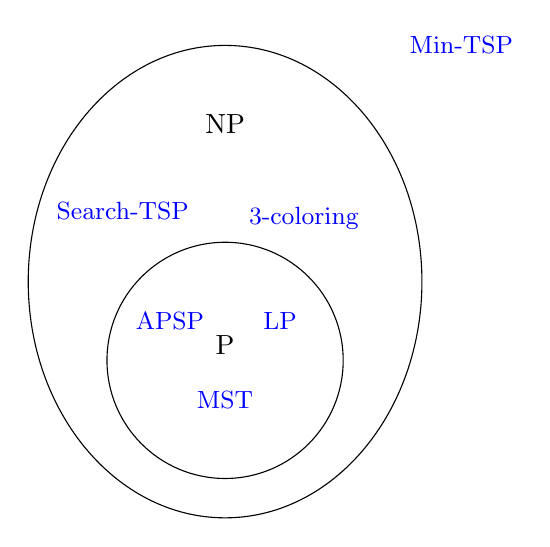
\begin{tikzpicture}
				\draw(0, 0) circle [radius=1.5cm];
				\draw node at (0, 0.2) {P};
				\draw (0, 1) ellipse [x radius = 2.5, y radius = 3];
				\draw node at (0, 3) {NP};
				\draw[blue] node at (0, -0.5) {\small MST};
				\draw[blue] node at (0.7, 0.5) {\small LP};
				\draw[blue] node at (-0.7, 0.5) {\small APSP};
				\draw[blue] node at (1, 1.8) {\small 3-coloring}; 
				\draw[blue] node at (-1.3, 1.9) {\small Search-TSP};
				\draw[blue] node at (3, 4) {\small Min-TSP};
			\end{tikzpicture}
		\end{center}
	\item We're not going to prove this, but it has been shown that factoring reduces to the 3-coloring 
		problem. Similarly, factoring also reduces to the Rudrata Cycle problem. 
	\item It turns out that every problem in NP reduces to Rudrata cycle!
	\item These are the most difficult problems in NP, and it can be shown that every problem in NP reduces 
		to an NP-complete problem
	\item \textbf{NP-Hardness:} A problem \(A\) is NP-hard if every problem \(B\) in NP reduces to \(A\). 
	\item \textbf{NP-Completeness:} A problelm \(A\) is NP-complete if \(A \in \text{NP}\) and \(A\) is 
		NP-hard.
	\item Problems in NP that aren't NP-complete are called an \textbf{NP-intermediate} problem 
	\item \textbf{Fact:} Given two problems that are NP-complete, then \(A \preceq_p B\) and \(B \preceq_p A\). 
		So this means that you can basically think of \(A\) and \(B\) are basically equivalent problems. 

		\question{Is this a biconditional?}

		\answer{No, consider two problems in P: they can be reduced to one another, but they are not 
		in NP.} 
		\begin{itemize}
			\item  There are thousands upon thousands of NP-complete problems, and by notion of reduction, 
				they are (in some sense) the same problem.
			\item This also means that if there exists a polynomial time algorithm for any NP-problem, 
				then this would imply that P = NP.
		\end{itemize}
		\question{How is it that if P = NP then every problem becomes NP-complete?}  
\end{itemize}

\subsection{Proving NP-Completeness}
\begin{itemize}
	\item Cook-Levin Theorem: showed that every problem in NP reduces in polynomial time to a circuit SAT 
		problem.
	\item It can then be shown that circuit-SAT reduces to 3-SAT, making 3-SAT an NP-complete problem. In 
		terms of a diagram:
		\begin{center}
			\begin{tikzpicture}[every text node part/.style={align=center}]
				\foreach \x in {0, 4}
						\draw[-stealth] (\x+0.5, 0) -- (\x+2, 0);
				\draw node at (-1, 0) {Every problem \\ in NP};
				\draw node at (3.25, 0) {Circuit\\SAT};
				\draw node at (7.25, 0) {3-SAT};
				\draw [-stealth] (8, 0) -- (10, 1.5) node[right] {Independent \\ Set};
				\draw [-stealth] (8, -0.2) -- (10, -1.5) node[right] {Rudrata Cycle};
			\end{tikzpicture}
		\end{center}
		\question{Finish this Diagram Later}
	\item To show that a problem is NP-complete, we first show that \(A \in \text{NP}\), then 
		pick some problem \(B\) that is known to be NP-complete and show that \(B \preceq_p A\). 
		
		\question{What if we show that \(A \preceq_p B\)?}

		\answer{We don't need to, since \(A \preceq_p B\) is true already because \(B\) 
		is an NP-complete problem!}
\end{itemize}
\subsection{Circuit SAT}
\begin{itemize}
	\item A Boolean circuit is a directed acyclic graph with:
		\begin{itemize}
			\item Input nodes \(x_1, \dots, x_n\) 
			\item one output node, with an output \(C(x)\)
			\item gates marked OR, AND, NOT: \(\lor, \land, \neg\)
		\end{itemize}
		A possible graph is:
		\begin{center}
			\begin{tikzpicture}
				\node (c) {$\lor$}
					child [stealth-] {node (a) [left] {$\land$}  
					child {node {$x_1 = 1$}}
				}
				child [stealth-] {node {$\land$}
				  child {node (b) {\(x_2 = 1\)} }
				  child {node {\(\neg\)} 
					  child {node {\(x_3 = 1\) }}
					}
				};
			\draw[-stealth] (b) -- (a);
			\draw[-stealth] (c) -- (0, 1) node[above]  {1}; 
			\end{tikzpicture}
		\end{center}	
	\item The input to circuit SAT is a circuit \(C\) with \(n\) inputs and \(m\) referring to the number of 
		gates. We want to output an assignment of \((x_1, \dots x_n)\) such that \(x_i \in \{0, 1\}\) 
		such that \(C(x) = 1\).
	\item By the Cook-Levin theorem, circuit-SAT is NP-complete. As for a bit of intuition on why this is true, 
		you can think of every problem as basically a collection of logical inputs, which basically means 
		that every problem can be reduced to some complex circuit of logical gates.  
\end{itemize}
\subsubsection{3-SAT}
\begin{itemize}
	\item Here, we're given \(n\) Boolean variables \( x_1, \dots, x_n\) such that \(x_i \in \{0, 1\} \), and 
		\(m \le  3\) variable clauses that join the variables together. 
	\item We want to output an assignment of \(x_1, \dots, x_n\) that satisfies all the clauses. 
	\item \textbf{Theorem:} Circuit-SAT reduces to 3-SAT

		\textit{Proof:} Suppose we're given an input to a circuit-SAT problem.
\end{itemize}

\end{document}
